\chapter{Software Framework}
\label{chapter: software}

\section{Firedrake}
\label{section:Firedrake}
As mentioned previously, one of the improvements Firedrake \cite{rathgeber2016firedrake} implemented over FEniCS \cite{alnaes2015fenics} is the creation of a new abstraction layer, namely PyOP2 \cite{rathgeber2012pyop2}, to distinguish between the local discretization or mathematical operators and their parallel execution over the mesh in the implementation layer. Firedrake models a finite problem as a combination of several abstractions---thereby allowing the user to follow a modularized approach while defining their problem.
 \begin{figure}[th]
        \centering
        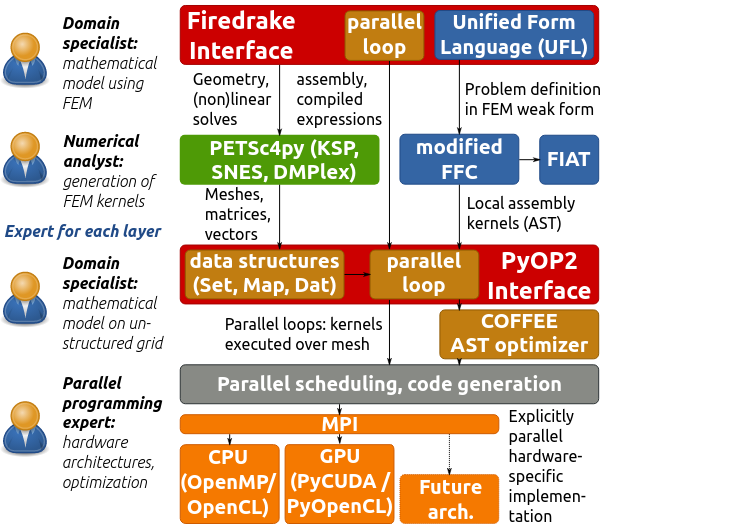
\includegraphics[width=0.8\textwidth]{figures/firedrake_toolchain_users.png}
        \caption{Firedrake Abstractions}Depiction of the separation of user concerns in Firedrake.Tools using FEniCS and PETSc are highlighted in blue and green respectively. The PyOP2 layers are shown in brown, while the backend engine is shown in orange \cite{rathgeber2016firedrake}.
        \label{figure:parameter}
        \end{figure}
As mentioned earlier, Firedrake improved upon FEniCS by adopting a philosophy that emphasized on the separation of concerns---thereby providing a clear distinction between the mathematical and programming aspects of the library. Since a multidisciplinary skillset, which ranges from mathematical expertise in numerical analyses to a deep understanding of parallel computation, is required for the development of these tools, it became more practical to develop abstract layers in the library that catered to a particular skillset. Firedrake introduced a new layer of abstraction named PyOP2 \cite{logg2010dolfin} that clearly formed a distinction between the finite element interface and the parallel execution of its algorithm over the mesh. PyOP2 thus creates a separation between the discretization of the mathematical operators and their parallel execution over the mesh. This has made the Firedrake codebase significantly more compact.  

The cost of typical finite element problems can be attributed to data movement and floating point operations---both of which are proportional to the mesh size. These operations can be divided into two categories---custom mesh-defined data structure iterations and sparse linear algebra. While Firedrake utilizes PETSc \cite{balay2001petsc} for the latter, PyOP2 was designed to address the former \cite{rathgeber2012pyop2}. Additional information regarding the integration of PyOP2 with the Firedrake layer is shown in the figure below \cite{rathgeber2016firedrake}.
\begin{figure}[th]
        \centering
        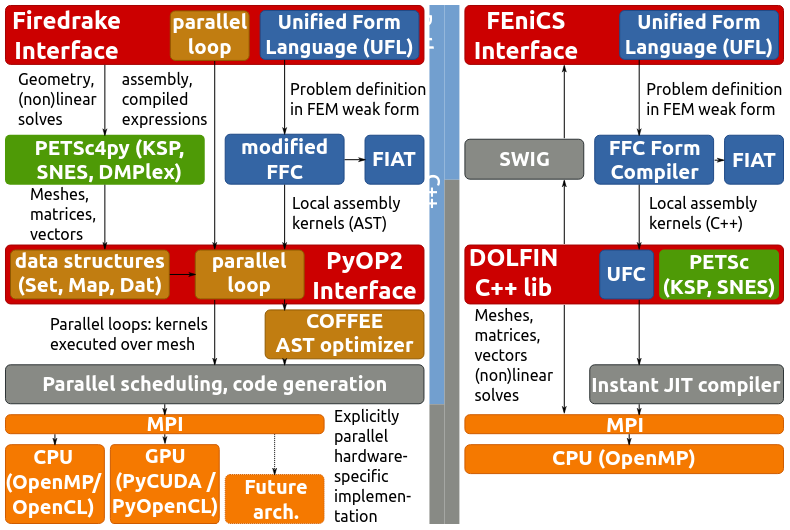
\includegraphics[width=0.8\textwidth]{figures/firedrake_toolchain_dolfin.png}
        \caption{Firedrake v/s FEniCS flow}The clear distinction introduced in Firedrake is evident from the PyOP2 interface in its flow. \cite{rathgeber2014firedrake}.
        \label{figure:parameter}
        \end{figure}

The primary motivation behind using Firedrake can be attributed to its improved abstraction layer. However, a comparative analysis of the performances of Firedrake and FEniCS was conducted \cite{rathgeber2016firedrake}. Firedrake reported a better performance than FEniCS---however, no concrete reason has been provided for its superior performance.


\section{ \texttt{hIPPYfire} }
\label{section:hIPPYfire}
\texttt{hIPPYfire} attempts to accomplish the same objective as that of \texttt{hIPPYlib} , i.e., implementation of scalable algorithms for PDE-based deterministic and Bayesian inverse problems. However, unlike its predecessor, it is built on Firedrake instead of FEniCS. The user is required to provide the PDE problem and likelihood in UFL \cite{alnaes2014unified}, and \texttt{hIPPYfire} computes the gradient and Hessian. \texttt{hIPPYfire} is currently in development and does not support all the functionality of \texttt{hIPPYlib} at the timing of writing this report. Its different components have been summarized below:
\begin{itemize}
    \item \textbf{Models}: The \texttt{modeling} module allows the user to specify information on the forward problem, misfit functional, and the prior. 
    \begin{enumerate}
        \item Forward Problem: This module computes the solutions of the forward, adjoint, and incremental problems. \texttt{hIPPYlib} and \texttt{hIPPYfire} both accept user input for the forward problem as a UFL form or user-defined object. The latter is required for transient inverse problems. However, if the forward problem is input as a UFL form, \texttt{hIPPYfire} computes the gradient and Hessian as well.
        \item Misfit: The misfit module evaluates the negative log-likelihood and its derivatives. Currently, the only misfit functional \texttt{hIPPYfire} provides support for is that of continuous observations---however, other functionals are currently in development.
        \item Prior: The prior computes the negative log-density and its derivatives, in addition to drawing samples and estimating the marginal variance. The user can select a Bilaplacian prior in \texttt{hIPPYfire}'s current implementation. There is a provision to accept user-defined priors as well.
        \item Model: The model is used to set up the \textit{p2o} map. Its three components are computed from the abovementioned modules.
        \item Hessian: If the forward problem is input in a standard UFL form, \texttt{hIPPYfire} internally computes the Hessian of the forward map. The collapse of the spectrum of the Hessian significantly influences the ill-posedness of the problem. However, the Hessian assumes a dense structure after discretization, thereby requiring forward and adjoint solves. Since the dimension of the Hessian is equal to that of the parameter, computing the Hessian for large-scale problems is not feasible. The rapidly decaying spectrum of the Hessian is exploited because the eigenvalues that tend to zero contain minimal information about the infinite-dimensional parameter field \cite{flath2011fast, bui2012analysis}.   
    \end{enumerate}  
    In case of transient problems, the user will have to provide their own derivatives.
    \item \textbf{Algorithms}: The \texttt{algorithms} module contains an implementation of the inexact Newton-CG algorithm \cite{borzi2011computational}. This is used to solve the deterministic inversion problem and compute the maximum \textit{a posteriori} distribution (also called the MAP point) for Bayesian inversion problems. Following the computation of the gradient and Hessian forms, the Newton system is solved according to the Steihaug criterion \cite{steihaug1983local}. Additional information regarding the implementation of this algorithm can be found in Villa et al. \cite{Villa2020}.  Custom linear algebra algorithms have also been implemented to perform basic matrix-vector operations that have been described later in this section.
    \item \textbf{Utilities}: The \texttt{utils} module contains certain helper functions to extract relevant data. The \texttt{vector2function} module wraps a discrete vector onto a continuous function, while the \texttt{rand} module generates random functions that are used to model the noise function and vector. The \texttt{parameterlist} module creates a custom list of parameters for the Newton solver.

    \begin{figure}[th]
        \centering
        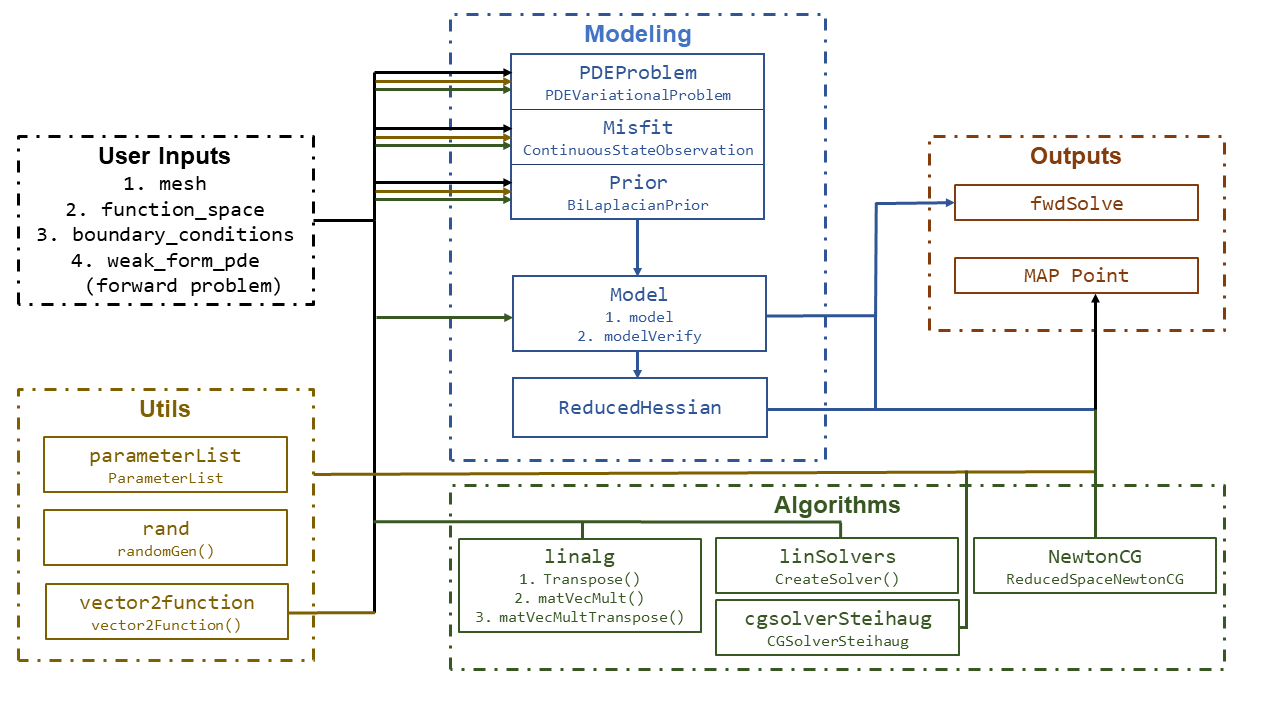
\includegraphics[width=1.0\textwidth]{figures/hIPPYfire.png}
        \caption{Flow and functionality of \texttt{hIPPYfire}}
        \label{figure:hippyfire}
    \end{figure}
    
    One of the major challenges faced in the development of \texttt{hIPPYfire} was the limited functionality of Firedrake's \texttt{firedrake.matrix.Matrix} data structure. Certain modules required matrix transpose and matrix-vector multiplication operations. Since these operations are not defined for the firedrake Matrix, Firedrake's interface with PETSc was used to create linear algebra operations between Firedrake objects and their PETSc wrappers. These operations include matrix transpose (\texttt{Transpose()}, matrix-vector multiplication (\texttt{matVecMult()}), and matrix-transpose-vector multiplication (\texttt{matVecMultTranspose()})---all of which have been defined in the \texttt{linalg} module. 
    The \texttt{hIPPYlib} library provides APIs to create different kinds of solvers (the \texttt{PETScKrylovSolver()} and \texttt{PETScLUSolver()}, \texttt{hIPPYfire} provides a single API (\texttt{CreateSolver()}), which acts as a wrapper for Firedrake's linear solvers API and allows the user to create their custom solver.
\end{itemize}